\ifx\wholebook\relax \else
% ------------------------

\documentclass[b5paper]{article}
\usepackage[nomarginpar
  %, margin=.5in
]{geometry}

\addtolength{\oddsidemargin}{-0.05in}
\addtolength{\evensidemargin}{-0.05in}
\addtolength{\textwidth}{0.1in}

\usepackage[en]{../../../prelude}

\setcounter{page}{1}

\begin{document}

\title{Red-black tree}

\author{Xinyu LIU
\thanks{{\bfseries Xinyu LIU} \newline
  Email: liuxinyu95@gmail.com \newline}
  }

\maketitle
\fi

\markboth{Red-black tree}{Elementary Algorithms}

\ifx\wholebook\relax
\chapter{Red-black tree}
\numberwithin{Exercise}{chapter}
\fi

\section{Introduction}
\label{sec:rbtree-introduction} \index{red-black tree}

As the example in chapter 2, we use the binary search tree as a dictionary to count the word occurrence in text. One may want to feed a address book to a binary search tree, and use it to look up the contact as below example program:

\lstset{frame = single}
\begin{lstlisting}[language=Bourbaki]
void addrBook(Input in) {
    bst<string, string> dict
    while (string name, string addr) = read(in) {
        dict[name] = addr
    }
    loop {
        string name = read(console)
        var addr = dict[name]
        if (addr == null) {
            print("not found")
        } else {
            print("address: ", addr)
        }
    }
}
\end{lstlisting}

Unlike the word counter program, this one performs poorly, especially when search names like Zara, Zed, Zulu, etc. This is because the address entries are typically listed in lexicographic order, i.e. the names are input in ascending order. If insert numbers 1, 2, 3, ..., $n$ to a binary search tree, it ends up like in figure \ref{fig:unbalanced-tree}. It is an extremely unbalanced binary search tree. The $lookup()$ is bound to $O(h)$ time for a tree with height $h$. When the tree is well balanced, the performance is $O(\lg n)$, where $n$ is the number of elements in the tree. But in this extreme case, the performance downgrades to $O(n)$. It is equivalent to list scan.

\begin{figure}[htbp]
  \centering
  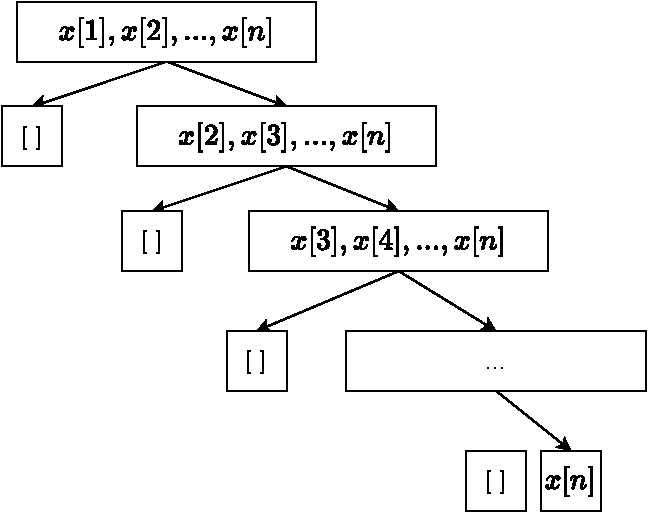
\includegraphics[scale=0.5]{img/unbalanced.ps}
  \caption{unbalanced tree}
  \label{fig:unbalanced-tree}
\end{figure}

\begin{Exercise}
\Question{For a big address entry list in lexicographic order, one may want to speed up building the address book with two concurrent tasks: one reads from the head; while the other reads from the tail, till they meet at some middle point. What does the binary search tree look like? What if split the list into multiple sections to scale the concurrency?}
\Question{Find more cases to exploit a binary search tree, for example in figure \ref{fig:unbalanced-trees}.}
\end{Exercise}

\begin{figure}[htbp]
  \centering
  \subcaptionbox{}{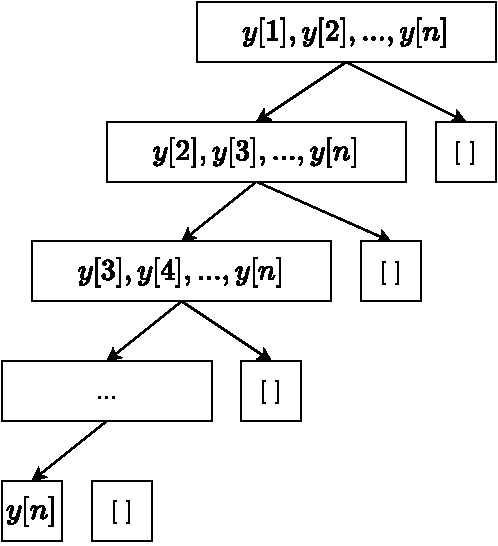
\includegraphics[scale=0.4]{img/unbalanced-2.ps}}
  \subcaptionbox{}{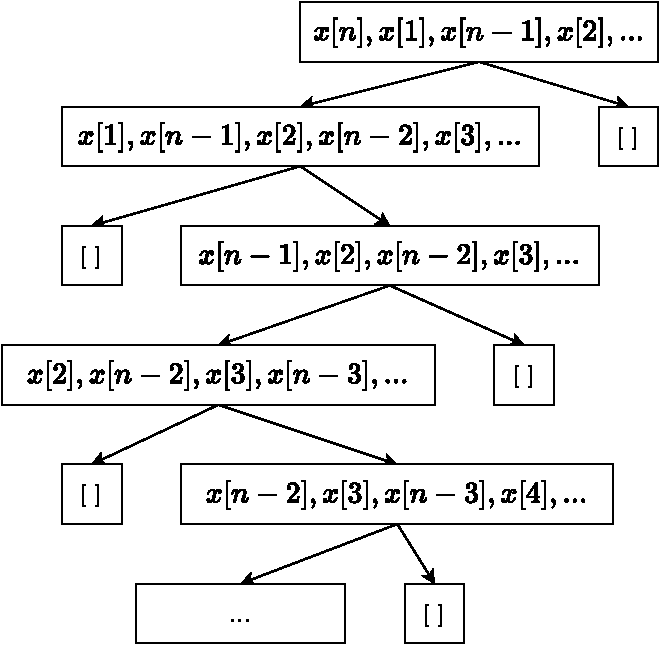
\includegraphics[scale=0.4]{img/unbalanced-zigzag.ps}} \\
  \subcaptionbox{}{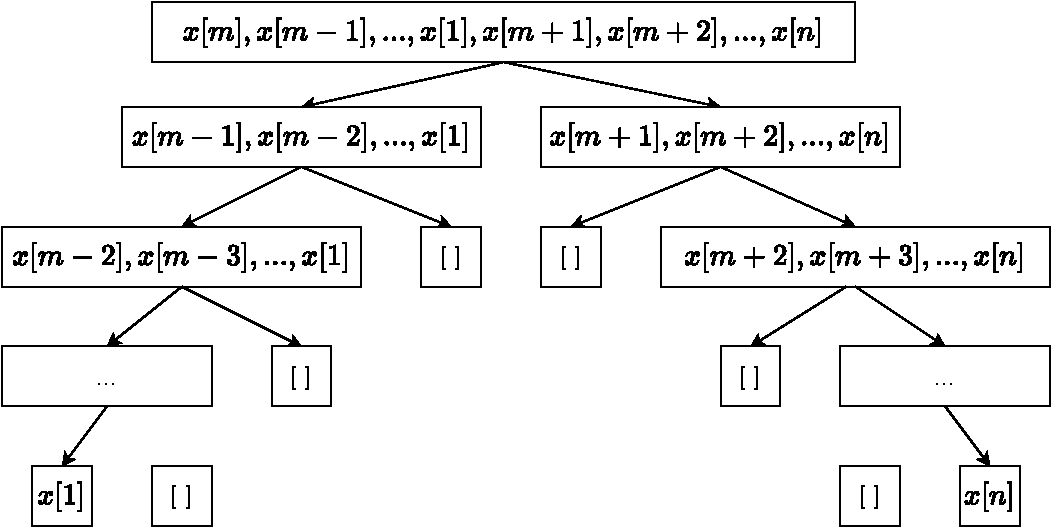
\includegraphics[scale=0.4]{img/unbalanced-3.ps}}
  \caption{Unbalanced trees}
  \label{fig:unbalanced-trees}
\end{figure}

\subsection{Balance}
To avoid extremely unbalanced case, we can shuffle the input(12.4 in \cite{CLRS}), however, when the input is entered by user interactively, we can not randomize the sequence. People developed solutions to make the tree balanced. They mostly rely on the rotation operation. Rotation changes the tree structure while maintain the elements ordering. This chapter introduces the red-black tree, the widely used self-adjusting balanced binary search tree. Next chapter is about AVL tree, another self-balanced tree. Chapter 8 introduce the splay tree. It adjusts the tree in steps to make it balanced.

\subsection{Tree rotation}
\index{tree rotation}

Tree rotation transforms the tree structure while keeping the in-order traverse result unchanged. There are multiple binary search trees generate the same ordered element sequence. Figure \ref{fig:tree-rotation} shows the tree rotation.

\begin{figure}[htbp]
   \centering
   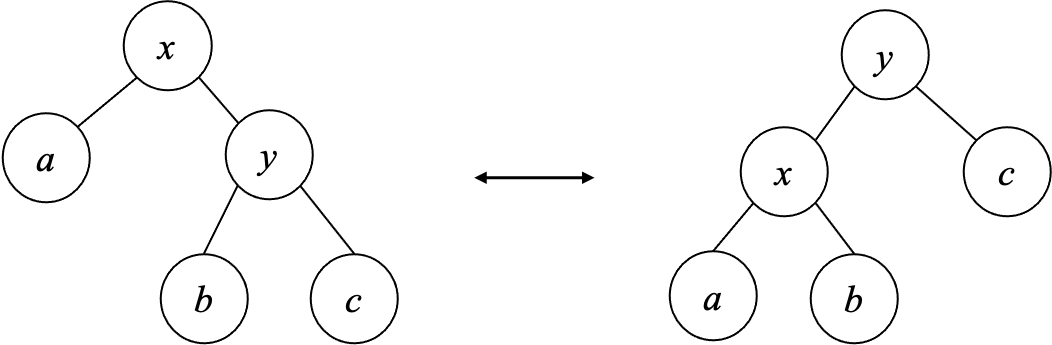
\includegraphics[scale=0.4]{img/tree-rotation.png}
   \caption{`left rotate' and `right rotate'.}
   \label{fig:tree-rotation}
\end{figure}

Tree rotation can be defined with pattern matching:

\be
\begin{array}{rcl}
rotate_l\ ((a, x, b), y, c) & = & (a, x, (b, y, c)) \\
rotate_l\ T & = & T \\
\end{array}
\ee

and

\be
\begin{array}{rcl}
rotate_r\ (a, x, (b, y, c)) & = & ((a, x, b), y, c)) \\
rotate_r\ T & = & T \\
\end{array}
\ee

The second row in each equation keeps the tree unchanged if the pattern does not match (for example, both sub-trees are empty). We can also implement tree rotation imperatively. We need re-assign sub-trees and parent node reference. When rotate, we pass both the root $T$, and the node $x$ as parameters:

\begin{algorithmic}[1]
\Function{Left-Rotate}{$T, x$}
  \State $p \gets$ \Call{Parent}{$x$}
  \State $y \gets$ \Call{Right}{$x$} \Comment{assume $y \ne$ NIL}
  \State $a \gets$ \Call{Left}{$x$}
  \State $b \gets$ \Call{Left}{$y$}
  \State $c \gets$ \Call{Right}{$y$}
  \State \Call{Replace}{$x, y$}  \Comment{replace node $x$ with $y$}
  \State \Call{Set-Subtrees}{$x, a, b$} \Comment{Set $a, b$ as the sub-trees of $x$}
  \State \Call{Set-Subtrees}{$y, x, c$} \Comment{Set $x, c$ as the sub-trees of $y$}
  \If{$p = $ NIL}  \Comment{$x$ was the root}
    \State $T \gets y$
  \EndIf
  \State \Return $T$
\EndFunction
\end{algorithmic}

The \textproc{Right-Rotate} is symmetric, we leave it as exercise. The \textproc{Replace}($x$, $y$) uses node $y$ to replace $x$:

\begin{algorithmic}[1]
\Function{Replace}{$x, y$}
  \State $p \gets$ \Call{Parent}{$x$}
  \If{$p$ = NIL} \Comment{$x$ is the root}
    \If{$y \ne$ NIL}
           \Call{Parent}{$y$} $\gets$ NIL
    \EndIf
  \ElsIf{\Call{Left}{$p$} $= x$}
    \State \Call{Set-Left}{$p$, $y$}
  \Else
    \State \Call{Set-Right}{$p$, $y$}
  \EndIf
  \State \Call{Parent}{$x$} $\gets$ NIL
\EndFunction
\end{algorithmic}

Procedure \textproc{Set-Subtrees}($x, L, R$) assigns $L$ as the left, and $R$ as the right sub-trees of $x$:

\begin{algorithmic}[1]
\Function{Set-Subtrees}{$x, L, R$}
  \State \Call{Set-Left}{$x, L$}
  \State \Call{Set-Right}{$x, R$}
\EndFunction
\end{algorithmic}

It further calls \textproc{Set-Left} and \textproc{Set-Right} to set the two sub-trees:

\begin{algorithmic}[1]
\Function{Set-Left}{$x, y$}
  \State \Call{Left}{$x$} $\gets y$
  \If{$y \ne$ NIL}
    \Call{Parent}{$y$} $\gets x$
  \EndIf
  \EndFunction

\Statex

\Function{Set-Right}{$x, y$}
  \State \Call{Right}{$x$} $\gets y$
  \If{$y \ne$ NIL}
    \Call{Parent}{$y$} $\gets x$
  \EndIf
\EndFunction
\end{algorithmic}

We can see how pattern matching simplifies the tree rotation. Based on this idea, Okasaki developed the purely functional algorithm for red-black tree in 1995\cite{okasaki}.

\begin{Exercise}
\Question{Implement the \textproc{Right-Rotate}.}
\end{Exercise}

\section{Definition}
\index{red-black tree}

A red-black tree is a self-balancing binary search tree\cite{wiki-rbt}. It is essentially equivalent to 2-3-4 tree\footnote{Chapter 7, B-tree. For any 2-3-4 tree, there is at least one red-black tree has the same ordered data.}. By coloring the node red or black, and performing rotation, red-black tree provides an efficient way to keep the tree balanced. On top of the binary search tree definition, we label the node with a color. We say it is a red-black tree if the coloring satisfies the following 5 rules(\cite{CLRS} pp273):

\index{red-black tree!red-black properties}
\begin{enumerate}
\item Every node is either red or black.
\item The root is black.
\item Every leaf (NIL) is black.
\item If a node is red, then both sub-trees are black.
\item For every node, all paths from it to descendant leaves contain the same number of black nodes.
\end{enumerate}

Why do they keep the red-black tree balanced? The key point is that, the longest path from the root to leaf can not be as 2 times longer than the shortest path. Consider rule 4, there can not be any two adjacent red nodes. Therefore, the shortest path only contains black nodes. Any longer path must have red ones. In addition, rule 5 ensures all paths have the same number of black nodes. So as to the root. It eventually ensures any path is not 2 times longer than others\cite{wiki-rbt}. Figure \ref{fig:rbt-example-with-nil} gives an example of red-black tree.

\begin{figure}[htbp]
  \centering
  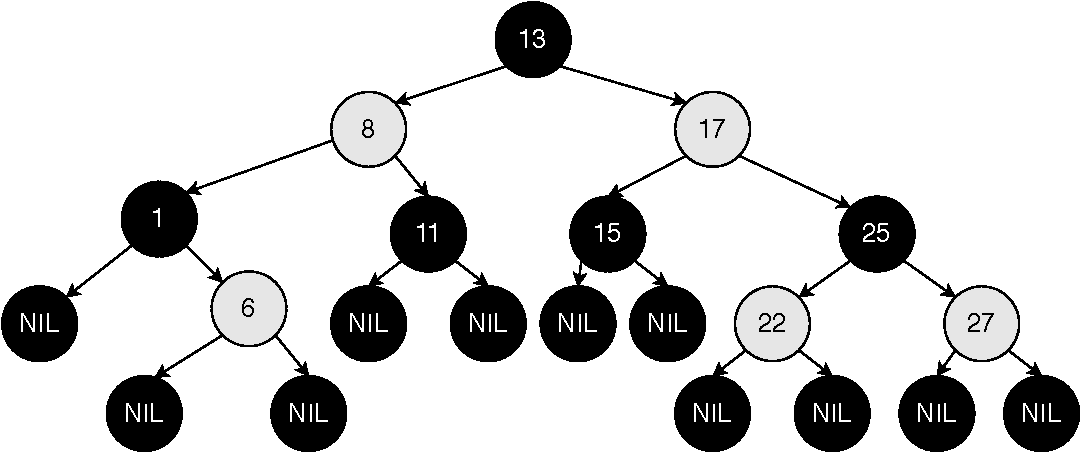
\includegraphics[scale=0.6]{img/rbt-example-with-nil.ps}
  \caption{A red-black tree}
  \label{fig:rbt-example-with-nil}
\end{figure}

As all NIL nodes are black, we can hide them as shown in figure \ref{fig:rbt-example}. All operations including $lookup$, $min/max$, are same as the binary search tree. However, the $insert$ and $delete$ are special, as we need maintain the coloring rules.

\begin{figure}[htbp]
  \centering
  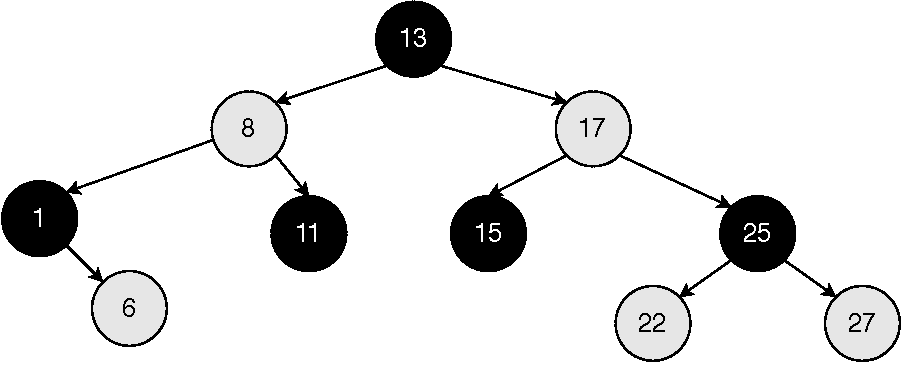
\includegraphics[scale=0.6]{img/rbt-example.ps}
  \caption{Hide the NIL nodes}
  \label{fig:rbt-example}
\end{figure}

Below example program adds the color field atop binary search tree definition:

\begin{Haskell}
data Color = R | B
data RBTree a = Empty
              | Node Color (RBTree a) a (RBTree a)
\end{Haskell}

\begin{Exercise}
\Question{Prove the height $h$ of a red-black tree of $n$ nodes is at most $2 \lg (n+1)$}
\end{Exercise}

\section{Insert}
\index{red-black tree!insert}

The $insert$ algorithm for red-black tree has two steps. The first step is as same as the binary search tree. The tree may become unbalanced after that, we need fix it to resume the red-black tree coloring in the second step. When insert a new element, we always make it red. Unless the new node is the root, we won't break any coloring rules except for the 4-th. Because it may bring two adjacent red nodes. Okasaki finds there are 4 cases violate rule 4. All have two adjacent red nodes. They share a uniformed structure after fixing\cite{okasaki} as shown in figure \ref{fig:insert-fix}.

\begin{figure}[htbp]
  \centering
  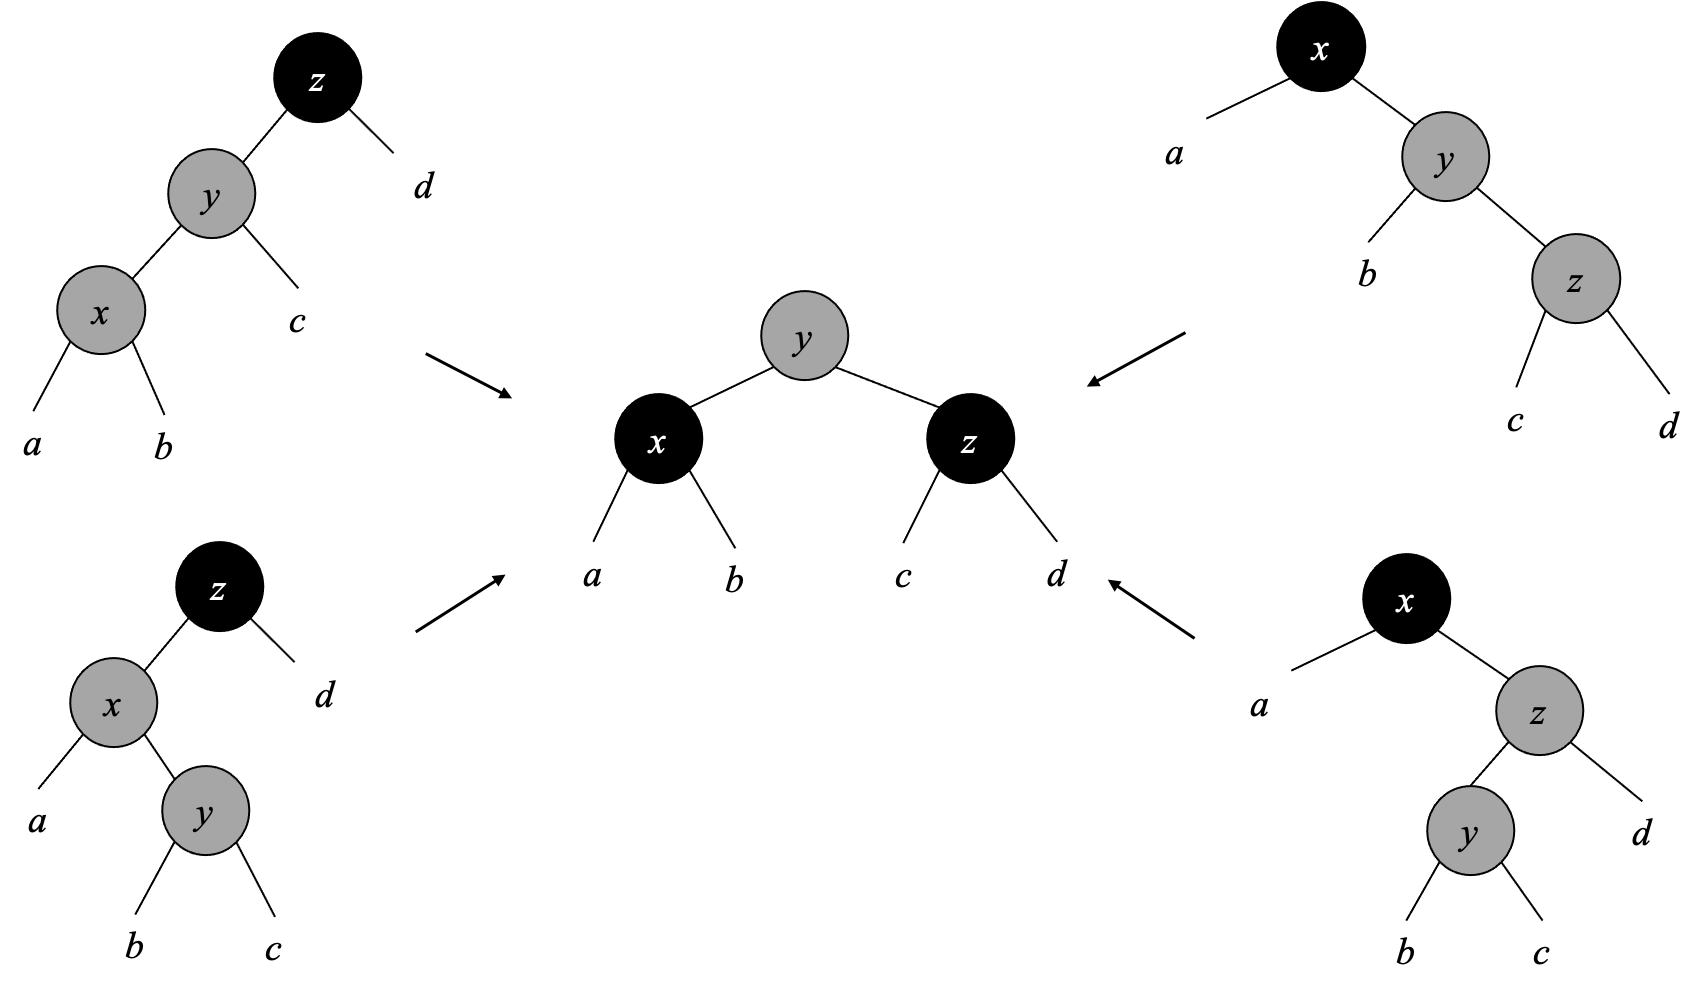
\includegraphics[scale=0.4]{img/insert-fix.png}
  \caption{Fix 4 cases to the same structure.}
  \label{fig:insert-fix}
\end{figure}

All 4 transformations move the redness one level up. When perform bottom-up recursive fixing, it may color the root red. While rule 2 requires the root always be black. We need revert the root back to black finally. With pattern matching, we can define a $balance$ function to fix the tree. Denote the color as $\mathcal{C}$ with values black $\mathcal{B}$, and red $\mathcal{R}$. A none empty node is in the form of $T = (\mathcal{C}, l, k, r)$, where $l, r$ are the left and right sub-trees, $k$ is the key.

\be
\begin{array}{rcl}
%\text{up left:} & & \\
balance\ \mathcal{B}\ (\mathcal{R}, (\mathcal{R}, a, x, b), y, c)\ z\ d & = & (\mathcal{R}, (\mathcal{B}, a, x, b), y, (\mathcal{B}, c, z, d)) \\
%\text{up right:} & & \\
balance\ \mathcal{B}, (\mathcal{R}, a, x, (\mathcal{R}, b, y, c))\ z\ d  & = & (\mathcal{R}, (\mathcal{B}, a, x, b), y, (\mathcal{B}, c, z, d)) \\
%\text{bottom left:} & & \\
balance\ \mathcal{B}\ a\ x\ (\mathcal{R}, b, y, (\mathcal{R}, c, z, d)) & = & (\mathcal{R}, (\mathcal{B}, a, x, b), y, (\mathcal{B}, c, z, d))  \\
%\text{bottom right:} & & \\
balance\ \mathcal{B}\ a\ x\ (\mathcal{R}, (\mathcal{R}, b, y, c), z, d) & = & (\mathcal{R}, (\mathcal{B}, a, x, b), y, (\mathcal{B}, c, z, d))  \\
%\text{otherwise:} & & \\
balance\ T & = & T \\
\end{array}
\ee

The last row says if the tree is not in any 4 patterns, then we leave it unchanged. We define the $insert$ algorithm for red-black tree as below:

\be
insert\ T\ k = makeBlack\ (ins\ T\ k)
\ee

where

\be
\begin{array}{rcl}
ins\ \nil\ k & = & (\mathcal{R}, \nil, k, \nil) \\
ins\ (\mathcal{C}, l, k', r)\ k & = & \begin{cases}
  k < k': & balance\ \mathcal{C}\ (ins\ l\ k)\ k'\ r \\
  k > k': & balance\ \mathcal{C}\ l\ k'\ (ins\ r\ k) \\
  \end{cases}
\end{array}
\ee

If the tree is empty, we create a red leaf of $k$; otherwise, let the sub-trees and the key be $l$, $r$, $k'$, we compare $k$ and $k'$, then recursively insert $k$ to a sub-tree. After that, we call $balance$ to fix the coloring, then force the root to be black finally.

\be
makeBlack\ (\mathcal{C}, l, k, r) = (\mathcal{B}, l, k, r)
\ee

Below is the corresponding example program:

\begin{Haskell}
insert t x = makeBlack $ ins t where
    ins Empty = Node R Empty x Empty
    ins (Node color l k r)
        | x < k     = balance color (ins l) k r
        | otherwise = balance color l k (ins r)
    makeBlack(Node _ l k r) = Node B l k r

balance B (Node R (Node R a x b) y c) z d =
                Node R (Node B a x b) y (Node B c z d)
balance B (Node R a x (Node R b y c)) z d =
                Node R (Node B a x b) y (Node B c z d)
balance B a x (Node R b y (Node R c z d)) =
                Node R (Node B a x b) y (Node B c z d)
balance B a x (Node R (Node R b y c) z d) =
                Node R (Node B a x b) y (Node B c z d)
balance color l k r = Node color l k r
\end{Haskell} %$

We skip to handle the duplicated keys. If the key already exists, we can overwrite, drop, or store the values in a list (\cite{CLRS}, pp269). Figure \ref{fig:insert-example} shows two red-black trees built from sequence 11, 2, 14, 1, 7, 15, 5, 8, 4 and 1, 2, ..., 8. The second example demonstrates the tree is well balanced even for ordered input.

\begin{figure}[htbp]
  \centering
  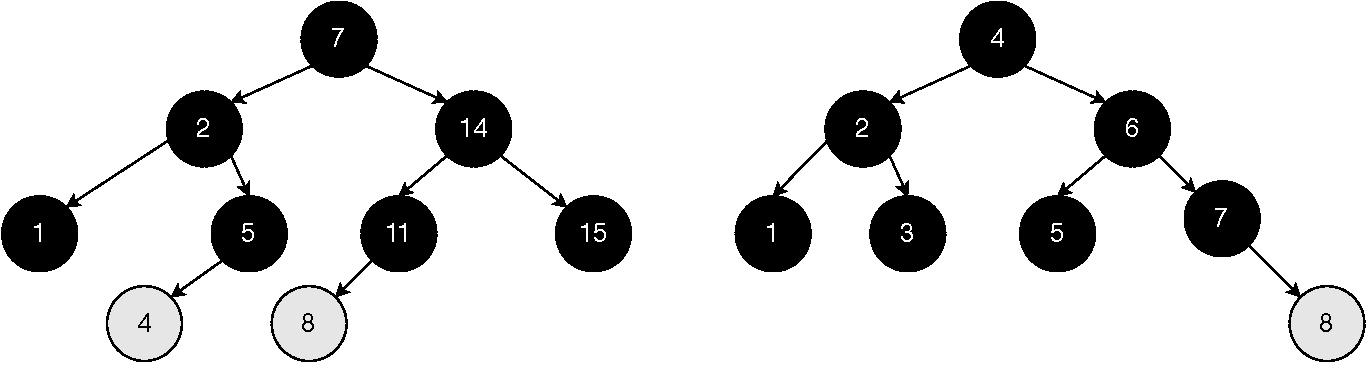
\includegraphics[scale=0.6]{img/insert-haskell.ps}
  \caption{Red-black tree examples}
  \label{fig:insert-example}
\end{figure}

The algorithm performs top-down recursive insertion and fixing. It is bound to $O(h)$ time, where $h$ is the height of the tree. As the red-black tree coloring rules are maintained, $h$ is the logarithm to the number of nodes $n$. The overall performance is $O(\lg n)$.

\begin{Exercise}
\Question{Implement the $insert$ algorithm without using pattern matching, but test the 4 cases separately.}
\end{Exercise}

\section{Delete}
\index{red-black tree!delete}

Delete is more complex than insert. We can also use pattern matching and recursion to simplify the $delete$ algorithm for red-black tree\footnote{Actually, the tree is rebuilt in purely functional setting, although the common part is reused. This feature is called `persist'}. There are alternatives to mimic delete. Sometimes, we build the read-only tree, then use it for frequently looking up\cite{okasaki-blog}. When delete, we mark the deleted node with a flag, and later rebuild the tree if such nodes exceeds 50\%. Delete may also violate the red-black tree coloring rules. We use the same idea to apply fixing after delete. The coloring violation only happens when delete a black node according to rule 5. The black nodes along the path decreases by one, hence not all paths contain the same number of black nodes.

To resume the blackness, we introduce a special `doubly-black' node(\cite{CLRS}, pp290). One such node is counted as 2 black nodes. When delete a black node $x$, we can move the blackness either up to its parent or down to one sub-tree. Let this node be $y$ that accepts the blackness. If $y$ was red, we turn it black; if $y$ was already black, we make it `doubly-black', denoted as $\mathcal{B}^2$. Below example program adds the `doubly-black' support:

\begin{Haskell}
data Color = R | B | BB
data RBTree a = Empty | BBEmpty
              | Node Color (RBTree a) a (RBTree a)
\end{Haskell}

Because all empty leaves are black, when push the blackness down to a leaf, it becomes `doubly-black' empty (\texttt{BBEmpty}, or bold $\pmb{\varnothing}$). The first step is to perform the normal binary search tree delete; then if the cut off node is black, we shift the blackness, and fix the tree coloring.

\be
delete = makeBlack \circ del
\ee

This definition is in Curried form. When delete the only element, the tree becomes empty. To cover this case, we modify $makeBlack$ as below:

\be
\begin{array}{rcl}
makeBlack\ \nil & = & \nil \\
makeBlack\ (\mathcal{C}, l, k, r) & = & (\mathcal{B}, l, k, r) \\
\end{array}
\ee

Where $del$ accepts the tree and $k$ to be deleted:

\be
\begin{array}{rcl}
del\ \nil\ k & = & \nil \\
del\ (\mathcal{C}, l, k', r)\ k & = & \begin{cases}
  k < k': & fixB^2(\mathcal{C}, (del\ l\ k), k', r) \\
  k > k': & fixB^2(\mathcal{C}, l, k', (del\ r\ k)) \\
  k = k': & \begin{cases}
    l = \nil: & (\mathcal{C} = \mathcal{B} \mapsto shiftB\ r, r) \\
    r = \nil: & (\mathcal{C} = \mathcal{B} \mapsto shiftB\ l, l) \\
    else: & fixB^2(\mathcal{C}, l, k'', (del\ r\ k'')) \\
    & \text{where}\ k'' = min(r) \\
  \end{cases}
\end{cases}
\end{array}
\ee

When the tree is empty, the result is $\nil$; otherwise, we compare the key $k'$ in the tree with $k$. If $k < k'$, we recursively
delete $k$ from the left sub-tree; if $k > k'$ then delete from the right. Because the recursive result may contain doubly-black node, we need apply $fixB^2$ to fix it. When $k = k'$, we need splice it out. If either sub-tree is empty, we replace it with the other, then shift the blackness if the spliced node is black. This is represented with McCarthy form $(p \mapsto a, b)$, which is equivalent to `(if $p$ then $a$ else $b$)'. If neither sub-tree is empty, we cut the minimum element $k'' = min(r)$, and use $k''$ to replace $k$.

To reserve the blackness, $shiftB$ makes a black node doubly-black, and forces it black for other cases. It flips doubly-black to normal black when applied twice.

\be
\begin{array}{rcl}
shiftB\ (\mathcal{B}, l, k, r) & = & (\mathcal{B}^2, l, k, r) \\
shiftB\ (\mathcal{C}, l, k, r) & = & (\mathcal{B}, l, k, r) \\
shiftB\ \nil & = & \pmb{\nil} \\
shiftB\ \pmb{\nil} & = & \nil \\
\end{array}
\ee

Below is the example program (except the doubly-black fixing part).

\begin{Haskell}
delete :: (Ord a) => RBTree a -> a -> RBTree a
delete t k = makeBlack $ del t k where
    del Empty _ = Empty
    del (Node color l k' r) k
        | k < k' = fixDB color (del l k) k' r
        | k > k' = fixDB color l k' (del r k)
        | isEmpty l = if color == B then shiftBlack r else r
        | isEmpty r = if color == B then shiftBlack l else l
        | otherwise = fixDB color l k'' (del r k'') where k''= min r
    makeBlack (Node _ l k r) = Node B l k r
    makeBlack _ = Empty

shiftBlack (Node B l k r) = Node BB l k r
shiftBlack (Node _ l k r) = Node B  l k r
shiftBlack Empty = BBEmpty
shiftBlack BBEmpty = Empty
\end{Haskell}

The $fixB^2$ function eliminates the doubly-black node by rotation and re-coloring. The doubly-black node can be branch node or empty $\pmb{\varnothing}$. There are three cases:

\textbf{Case 1}. {\em The sibling of the doubly-black node is black, and it has a red sub-tree.} We can fix this case with a rotation. There are 4 sub-cases, all can be transformed to a uniformed pattern, as shown in figure \ref{fig:del-case1}.

\begin{figure}[htbp]
  \centering
  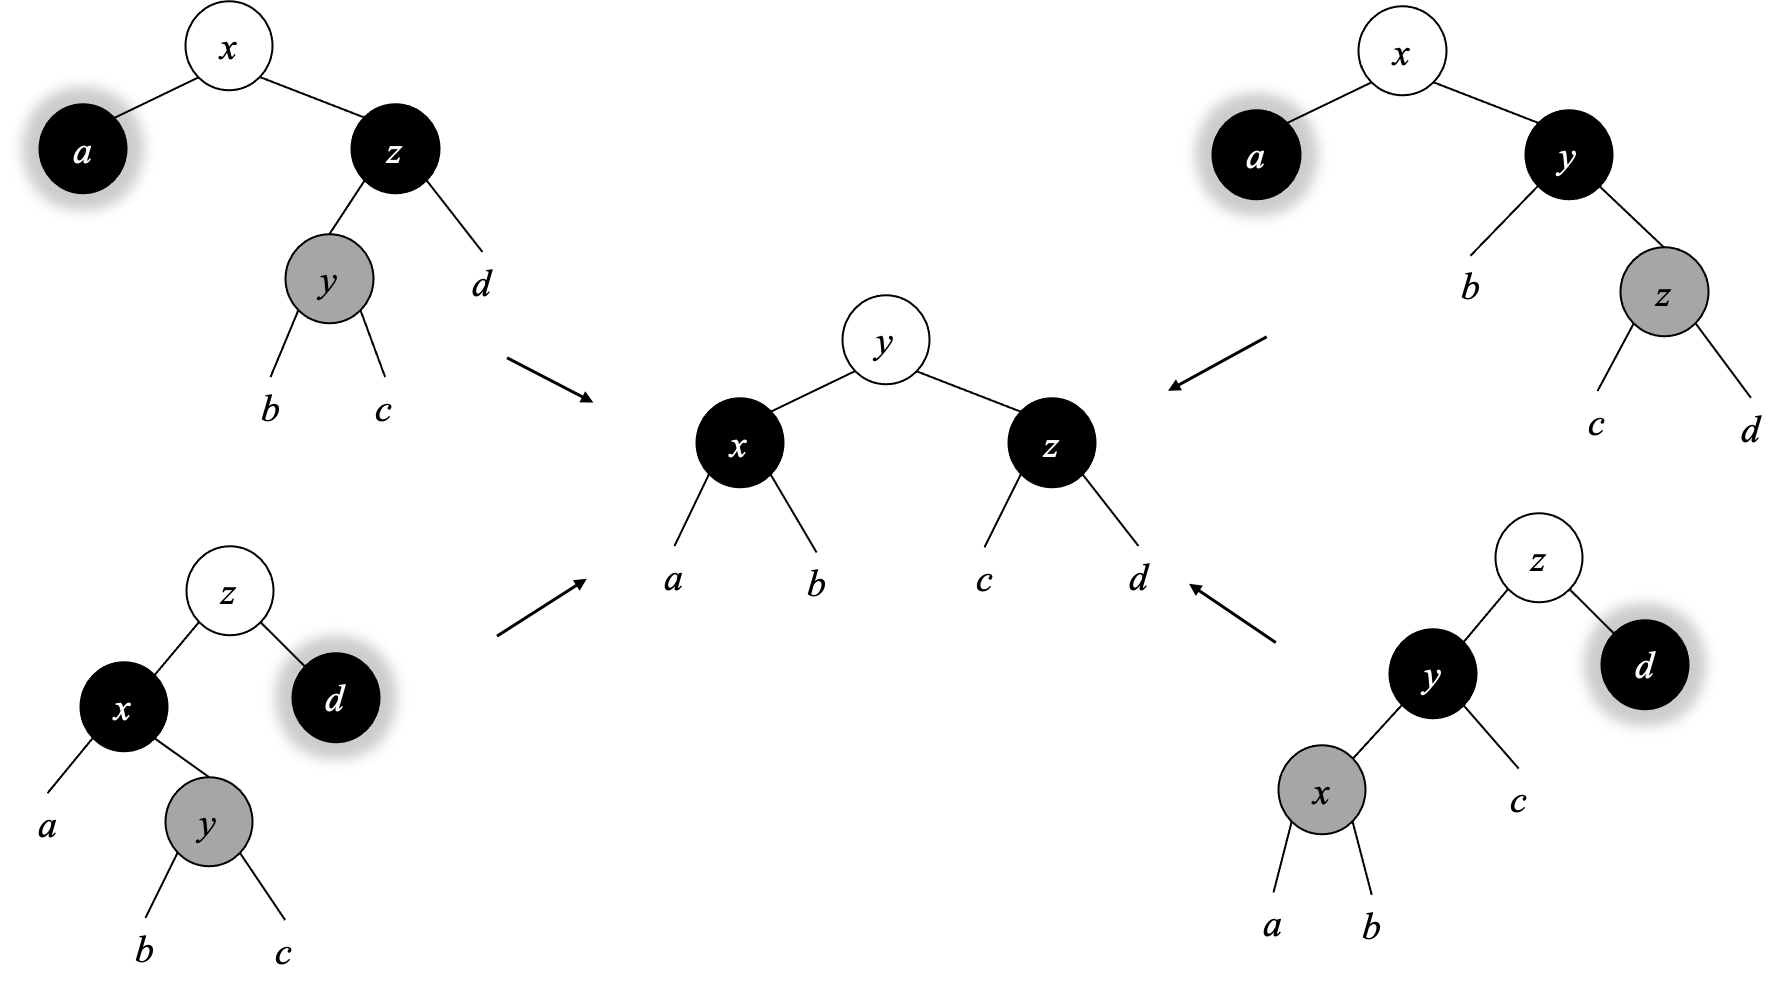
\includegraphics[scale=0.4]{img/del-case1.png}
  \caption{4 sub-cases share the uniformed fixing pattern}
  \label{fig:del-case1}
\end{figure}

The fixing for these 4 sub-cases can be realized with pattern matching.

\be
\resizebox{\textwidth}{!}{\ensuremath{
\begin{array}{rcl}
%\text{case 1 up left:} & & \\
fixB^2\ \mathcal{C}\ a_{\mathcal{B}^2}\ x\ (\mathcal{B}, (\mathcal{R}, b, y, c), z, d) & = & (\mathcal{C}, (\mathcal{B}, shiftB(a), x, b), y, (\mathcal{B}, c, z, d)) \\
%\text{case 1 up right:} & & \\
fixB^2\ \mathcal{C}\ a_{\mathcal{B}^2}\ x\ (\mathcal{B}, b, y, (\mathcal{R}, c, z, d)) & = & (\mathcal{C}, (\mathcal{B}, shiftB(a), x, b), y, (\mathcal{B}, c, z, d)) \\
%\text{case 1 bottom left:} & & \\
fixB^2\ \mathcal{C}\ (\mathcal{B}, a, x, (\mathcal{R}, b, y, c))\ z\ d_{\mathcal{B}^2} & = & (\mathcal{C}, (\mathcal{B}, a, x, b), y, (\mathcal{B}, c, z, shiftB(d))) \\
%\text{case 1 bottom right:} & & \\
fixB^2\ \mathcal{C}\ (\mathcal{B}, (\mathcal{R}, a, x, b), y, c)\ z\ d_{\mathcal{B}^2} & = & (\mathcal{C}, (\mathcal{B}, a, x, b), y, (\mathcal{B}, c, z, shiftB(d))) \\
\end{array}
}}
\label{eq:db-case-1}
\ee

Where $a_{\mathcal{B}^2}$ means node $a$ is doubly-black, it can be branch or $\pmb{\varnothing}$.

\textbf{Case 2}. {\em The sibling of the doubly-black is red.} We can rotate the tree to turn it into case 1 or 3, as shown in figure \ref{fig:del-case2}.

\begin{figure}[htbp]
  \centering
  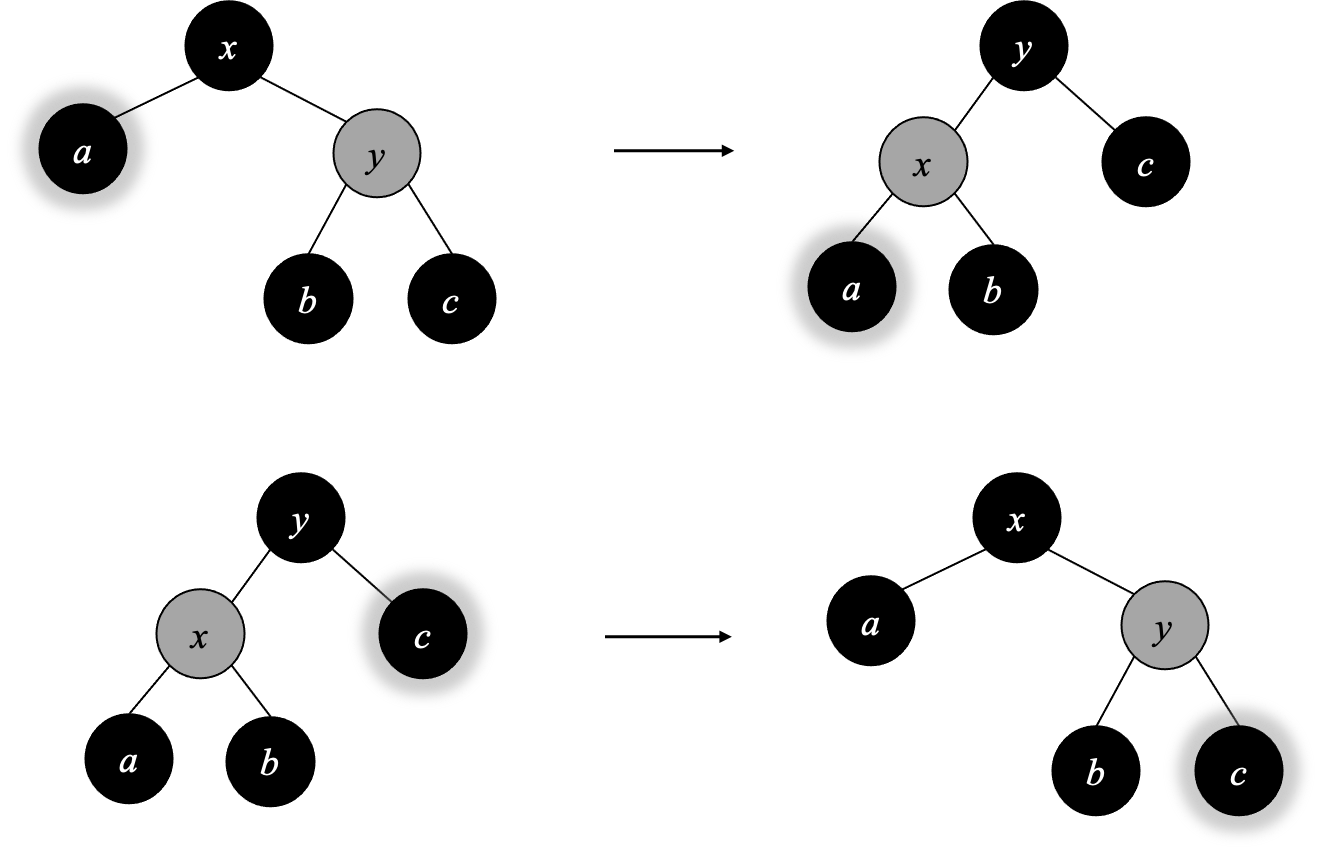
\includegraphics[scale=0.4]{img/del-case2.png}
  \caption{The sibling of the doubly-black is red.}
  \label{fig:del-case2}
\end{figure}

We add this fixing as additional 2 rows in equation (\ref{eq:db-case-1}):

\be
%\resizebox{\textwidth}{!}{\ensuremath{
\begin{array}{rcl}
\text{...} & & \\
%\text{case 2 up:} & & \\
fixB^2\ \mathcal{B}\ a_{\mathcal{B}^2}\ x\ (\mathcal{R}, b, y, c) & = & fixB^2\ \mathcal{B}\ (fixB^2\ \mathcal{R}\ a\ x\ b)\ y\ c \\
%\text{case 2 bottom:} & & \\
fixB^2\ \mathcal{B}\ (\mathcal{R}, a, x, b)\ y\ c_{\mathcal{B}^2} & = & fixB^2\ \mathcal{B}\ a\ x\ (fixB^2\ \mathcal{R}\ b\ y\ c)
\end{array}
%}}
\label{eq:db-case-2}
\ee

\textbf{Case 3}. {\em The sibling of the doubly-black node, and its two sub-trees are all black.} In this case, we change the sibling to red, flip the
doubly-black node to black, and propagate the doubly-blackness a level up to parent as shown in figure \ref{fig:del-case3}.

\begin{figure}[htbp]
  \centering
  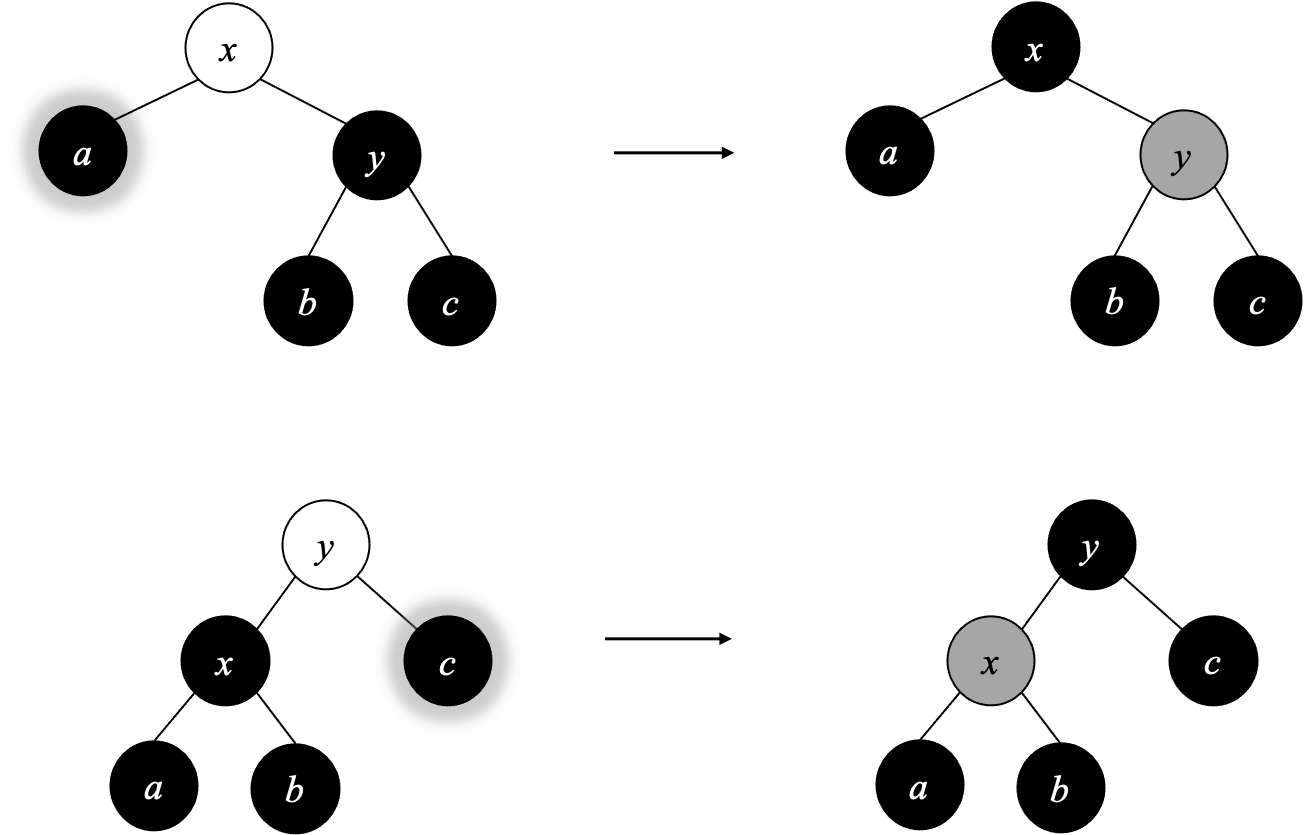
\includegraphics[scale=0.4]{img/del-case3.png}
  \caption{propagate the blackness up.}
  \label{fig:del-case3}
\end{figure}

There are two symmetric sub-cases. For the upper case, $x$ was either red or black. $x$ changes to black if it was red, otherwise changes to doubly-black; Same coloring changes to $y$ in the lower case. We add this fixing to equation (\ref{eq:db-case-2}):

\be
%\resizebox{\textwidth}{!}{\ensuremath{
\begin{array}{rcl}
\text{...} & & \\

fixB^2\ \mathcal{C}\ a_{\mathcal{B}^2}\ x\ (\mathcal{B}, b, y, c) & = & shiftB\ (\mathcal{C}, (shiftB\ a), x, (\mathcal{R}, b, y, c)) \\

fixB^2\ \mathcal{C}\ (\mathcal{B}, a, x, b)\ y\ c_{\mathcal{B}^2} & = & fixB^2\ \mathcal{B}\ a\ x\ (fixB^2\ \mathcal{R}\ b\ y\ c) \\

fixB^2\ \mathcal{C}\ l\ k\ r\ & = & (\mathcal{C}, l, k, r) \\
\end{array}
%}}
\label{eq:db-case-3}
\ee

If none of the patterns match, the last row keeps the node unchanged. The doubly-black fixing is recursive. It terminates in two ways: One is \textbf{Case 1}, the doubly-black node is eliminated. Otherwise the blackness may move up till the root. Finally the we force the root be black. Below example program puts all three cases together:

\begin{Haskell}
-- the sibling is black, and has a red sub-tree
fixDB color a@(Node BB _ _ _) x (Node B (Node R b y c) z d)
      = Node color (Node B (shiftBlack a) x b) y (Node B c z d)
fixDB color BBEmpty x (Node B (Node R b y c) z d)
      = Node color (Node B Empty x b) y (Node B c z d)
fixDB color a@(Node BB _ _ _) x (Node B b y (Node R c z d))
      = Node color (Node B (shiftBlack a) x b) y (Node B c z d)
fixDB color BBEmpty x (Node B b y (Node R c z d))
      = Node color (Node B Empty x b) y (Node B c z d)
fixDB color (Node B a x (Node R b y c)) z d@(Node BB _ _ _)
      = Node color (Node B a x b) y (Node B c z (shiftBlack d))
fixDB color (Node B a x (Node R b y c)) z BBEmpty
      = Node color (Node B a x b) y (Node B c z Empty)
fixDB color (Node B (Node R a x b) y c) z d@(Node BB _ _ _)
      = Node color (Node B a x b) y (Node B c z (shiftBlack d))
fixDB color (Node B (Node R a x b) y c) z BBEmpty
      = Node color (Node B a x b) y (Node B c z Empty)
-- the sibling is red
fixDB B a@(Node BB _ _ _) x (Node R b y c)
      = fixDB B (fixDB R a x b) y c
fixDB B a@BBEmpty x (Node R b y c)
      = fixDB B (fixDB R a x b) y c
fixDB B (Node R a x b) y c@(Node BB _ _ _)
      = fixDB B a x (fixDB R b y c)
fixDB B (Node R a x b) y c@BBEmpty
      = fixDB B a x (fixDB R b y c)
-- the sibling and its 2 children are all black, move the blackness up
fixDB color a@(Node BB _ _ _) x (Node B b y c)
      = shiftBlack (Node color (shiftBlack a) x (Node R b y c))
fixDB color BBEmpty x (Node B b y c)
      = shiftBlack (Node color Empty x (Node R b y c))
fixDB color (Node B a x b) y c@(Node BB _ _ _)
      = shiftBlack (Node color (Node R a x b) y (shiftBlack c))
fixDB color (Node B a x b) y BBEmpty
      = shiftBlack (Node color (Node R a x b) y Empty)
-- otherwise
fixDB color l k r = Node color l k r
\end{Haskell}

The delete algorithm is bound to $O(h)$ time, where $h$ is the height of the tree. As red-black tree maintains the balance, $h = O(\lg n)$ for $n$ nodes.

\begin{Exercise}
\Question{Implement the alternative delete algorithm: mark the node as deleted without actually removing it. When the marked nodes exceed 50\%, re-build the tree.}
\end{Exercise}

\section{Imperative red-black tree algorithm $\star$}
\index{red-black tree!imperative insertion}

We simplify the red-black tree implementation with pattern matching. In this section, we give the imperative algorithm for completeness. When insert, the first step is as same as the binary search tree, then as the second step, we fix the balance through tree rotations.

\begin{algorithmic}[1]
\Function{Insert}{$T, k$}
  \State $root \gets T$
  \State $x \gets$ \Call{Create-Leaf}{$k$}
  \State \Call{Color}{$x$} $\gets$ RED
  \State $p \gets$ NIL
  \While{$T \neq$ NIL}
    \State $p \gets T$
    \If{$k <$ \Call{Key}{$T$}}
      \State $T \gets $ \Call{Left}{$T$}
    \Else
      \State $T \gets $ \Call{Right}{$T$}
    \EndIf
  \EndWhile
  \State \Call{Parent}{$x$} $\gets p$
  \If{$p =$ NIL} \Comment{tree $T$ is empty}
    \State \Return $x$
  \ElsIf{$k <$ \Call{Key}{$p$}}
    \State \Call{Left}{$p$} $\gets x$
  \Else
    \State \Call{Right}{$p$} $\gets x$
  \EndIf
  \State \Return \Call{Insert-Fix}{$root, x$}
\EndFunction
\end{algorithmic}

We make the new node red, and then perform fixing before return. There are 3 basic cases, each one has a symmetric case, hence there are total 6 cases. Among them, we can merge two cases, because both have a red `uncle' node. We change the parent and uncle to black, and set grand parent to red:

\begin{algorithmic}[1]
\Function{Insert-Fix}{$T, x$}
  \While{\Call{Parent}{$x$} $\neq$ NIL and \textproc{Color}(\Call{Parent}{$x$}) = RED}
    \If{\textproc{Color}(\Call{Uncle}{$x$}) $=$ RED}
      \Comment{Case 1, $x$'s uncle is red}
      \State \textproc{Color}(\Call{Parent}{$x$}) $\gets$ BLACK
      \State \textproc{Color}(\Call{Grand-Parent}{$x$}) $\gets$ RED
      \State \textproc{Color}(\Call{Uncle}{$x$}) $\gets$ BLACK
      \State $x \gets$ \Call{Grand-Parent}{$x$}
    \Else
      \Comment{$x$'s uncle is black}
      \If{\Call{Parent}{$x$} = \textproc{Left}(\Call{Grand-Parent}{$x$})}
        \If{ $x =$ \textproc{Right}(\Call{Parent}{$x$})}
          \Comment{Case 2, $x$ is on the right}
          \State $x \gets$ \Call{Parent}{$x$}
          \State $T \gets$ \Call{Left-Rotate}{$T, x$}
        \EndIf
        \Comment{Case 3, $x$ is on the left}
        \State \textproc{Color}(\Call{Parent}{$x$}) $\gets$ BLACK
        \State \textproc{Color}(\Call{Grand-Parent}{$x$}) $\gets$ RED
        \State $T \gets$ \textproc{Right-Rotate}($T$, \Call{Grand-Parent}{$x$})
      \Else
        \If{ $x =$ \textproc{Left}(\Call{Parent}{$x$})}
          \Comment{Case 2, Symmetric}
          \State $x \gets$ \Call{Parent}{$x$}
          \State $T \gets$ \Call{Right-Rotate}{$T, x$}
        \EndIf
        \Comment{Case 3, Symmetric}
        \State \textproc{Color}(\Call{Parent}{$x$}) $\gets$ BLACK
        \State \textproc{Color}(\Call{Grand-Parent}{$x$}) $\gets$ RED
        \State $T \gets$ \textproc{Left-Rotate}($T$, \Call{Grand-Parent}{$x$})
      \EndIf
    \EndIf
  \EndWhile
  \State \Call{Color}{$T$} $\gets$ BLACK
  \State \Return $T$
\EndFunction
\end{algorithmic}

This algorithm takes $O(\lg n)$ time to insert a key, where $n$ is the number of nodes. Compare to the $balance$ function defined previously, they have different logic. Even input the same sequence of keys, they build different red-black trees. Figure \ref{fig:imperative-insert} shows the result when input the same sequence of keys to the imperative algorithm. We can see the difference from figure \ref{fig:insert-example}. There is a bit performance overhead in the pattern matching algorithm. Okasaki discussed the difference in detail in \cite{okasaki}.

\begin{figure}[htbp]
   \centering
   \includegraphics[scale=0.4]{img/clrs-fig-13-4.ps}
   \includegraphics[scale=0.4]{img/python-insert.ps}
   \caption{Red-black trees created by imperative algorithm.}
   \label{fig:imperative-insert}
\end{figure}

We provide the imperative delete algorithm in Appendix A of this book.

\section{Summary}
Red-black tree is a popular implementation of balanced binary search tree. We introduce another one, called AVL tree in the next chapter. Red-black tree is a good start for more data structures. If extend the number of children from 2 to $k$, and maintain the balance, it leads to B-tree; If store the data along with the edge but not inside node, it leads to Radix tree. To maintain the balance, we need handle multiple cases. Okasaki's developed a method that makes the red-black tree easy to implement. There are many implementations based on this idea\cite{rosetta}. We also provide AVL tree and Splay tree implementation based on pattern matching in this book.

\section{Appendix: Example programs}

Definition of red-black tree node with parent field. When not explicitly defined, the color of the new node is red by default.

\begin{lstlisting}[language = Bourbaki]
data Node<T> {
    T key
    Color color
    Node<T> left
    Node<T> right
    Node<T> parent

    Node(T x) = Node(null, x, null, Color.RED)

    Node(Node<T> l, T k, Node<T> r, Color c) {
        left = l, key = k, right = r, color = c
        if left != null then left.parent = this
        if right != null then right.parent = this
    }

    Self setLeft(l) {
        left = l
        if l != null then l.parent = this
    }

    Self setRight(r) {
        right = r
        if r != null then r.parent = this
    }

    Node<T> sibling() = if parent.left == this then parent.right
                        else parent.left

    Node<T> uncle() = parent.sibling()

    Node<T> grandparent() = parent.parent
}
\end{lstlisting}

Insert a key to red-black tree:

\begin{lstlisting}[language = Bourbaki]
Node<T> insert(Node<T> t, T key) {
    root = t
    x = Node(key)
    parent = null
    while (t != null) {
        parent = t
        t = if (key < t.key) then t.left else t.right
    }
    if (parent == null) {    //tree is empty
        root = x
    } else if (key < parent.key) {
        parent.setLeft(x)
    } else {
        parent.setRight(x)
    }
    return insertFix(root, x)
}
\end{lstlisting}

Fix the balance:

\begin{lstlisting}[language = Bourbaki]
// Fix the red->red violation
Node<T> insertFix(Node<T> t, Node<T> x) {
    while (x.parent != null and x.parent.color == Color.RED) {
        if (x.uncle().color == Color.RED) {
            // case 1: ((a:R x:R b) y:B c:R) ==> ((a:R x:B b) y:R c:B)
            x.parent.color = Color.BLACK
            x.grandparent().color = Color.RED
            x.uncle().color = Color.BLACK
            x = x.grandparent()
        } else {
            if (x.parent == x.grandparent().left) {
                if (x == x.parent.right) {
                    // case 2: ((a x:R b:R) y:B c) ==> case 3
                    x = x.parent
                    t = leftRotate(t, x)
                }
                // case 3: ((a:R x:R b) y:B c) ==> (a:R x:B (b y:R c))
                x.parent.color = Color.BLACK
                x.grandparent().color = Color.RED
                t = rightRotate(t, x.grandparent())
            } else {
                if (x == x.parent.left) {
                    // case 2': (a x:B (b:R y:R c)) ==> case 3'
                    x = x.parent
                    t = rightRotate(t, x)
                }
                // case 3': (a x:B (b y:R c:R)) ==> ((a x:R b) y:B c:R)
                x.parent.color = Color.BLACK
                x.grandparent().color = Color.RED
                t = leftRotate(t, x.grandparent())
            }
        }
    }
    t.color = Color.BLACK
    return t
}
\end{lstlisting}

\ifx\wholebook\relax \else
\begin{thebibliography}{99}

\bibitem{CLRS}
Thomas H. Cormen, Charles E. Leiserson, Ronald L. Rivest and Clifford Stein.
``Introduction to Algorithms, Second Edition''. ISBN:0262032937. The MIT Press. 2001

\bibitem{okasaki}
Chris Okasaki. ``FUNCTIONAL PEARLS Red-Black Trees in a Functional Setting''. J. Functional Programming. 1998

\bibitem{okasaki-blog}
Chris Okasaki. ``Ten Years of Purely Functional Data Structures''. \url{http://okasaki.blogspot.com/2008/02/ten-years-of-purely-functional-data.html}

\bibitem{wiki-rbt}
Wikipedia. ``Red-black tree''. \url{http://en.wikipedia.org/wiki/Red-black\_tree}

\bibitem{rosetta}
Pattern matching. \url{http://rosettacode.org/wiki/Pattern\_matching}

\end{thebibliography}

\expandafter\enddocument
\fi
